\documentclass[aspectratio=169,10pt]{beamer}

\usetheme{Madrid}
\usecolortheme{default}
\setbeamertemplate{navigation symbols}{}
\setbeamertemplate{footline}[frame number]

\usepackage{amsmath,amssymb,amsthm,booktabs,mathtools}
\usepackage{graphicx}
\usepackage{hyperref}
\usepackage{tikz}
\usetikzlibrary{arrows.meta,positioning,decorations.pathreplacing,fit}

\definecolor{positive}{HTML}{0173B2}
\definecolor{negative}{HTML}{DE8F05}
\definecolor{emphasis}{HTML}{029E73}
\definecolor{neutral}{gray}{0.55}
\definecolor{cbPurple}{HTML}{CC78BC}
\newcommand{\pos}[1]{\textcolor{positive}{#1}}
\newcommand{\con}[1]{\textcolor{negative}{#1}}
\newcommand{\HL}[1]{\textcolor{emphasis}{#1}}
\setbeamercolor{alerted text}{fg=negative}
\setbeamercolor{block title alerted}{fg=white,bg=negative}
\setbeamercolor{block body alerted}{fg=black,bg=negative!8}
\setbeamercolor{block title example}{fg=white,bg=emphasis}
\setbeamercolor{block body example}{fg=black,bg=emphasis!8}

\newcommand{\M}{\mathcal M}
\newcommand{\R}{\mathbb R}
\newcommand{\Y}{\mathcal Y}
\newcommand{\N}{\mathcal N}
\newcommand{\dist}{\operatorname{dist}}
\newcommand{\Cov}{\operatorname{Cov}}

\title[Inferring manifolds with GPs]{Inferring Manifolds Using Gaussian Processes}
\subtitle{From noisy local geometry to probabilistic reconstruction}
%\author{Presenter: Yiqing Sun}
%\institute{National University of Singapore}
\date{}

\begin{document}

\begin{frame}
  \titlepage
  \vspace{-0.4cm}
  \begin{center}
    \small Based on Dunson and Wu, \emph{Biometrika} (2026)
  \end{center}
\end{frame}

\section{Motivation}

\begin{frame}{Dimension reduction is not manifold reconstruction}
  \begin{columns}[T]
    \column{0.48\textwidth}
      \begin{block}{Classical manifold learning}
        \[
          y_i\in\R^D \longmapsto z_i\in\R^d
        \]
      \end{block}
      \begin{itemize}
        \item coordinates for visualization or downstream learning
        \item manifold between observations: \con{not estimated}
        \item original data: \con{not denoised}
      \end{itemize}
    \column{0.48\textwidth}
      \begin{exampleblock}{Manifold estimation}
        \[
          \{y_i\}_{i=1}^n \longmapsto \{\hat{y_i}\}_{i=1}^n\in \widehat{\M}\subset\R^D
        \]
      \end{exampleblock}
      \begin{itemize}
        \item fitted values in the ambient space
        \item interpolation between observations
        \item local structures: tangent space or curvature
      \end{itemize}
  \end{columns}
\end{frame}

\begin{frame}{Statistical target of MrGap}
  Observations fluctuate around an unknown embedded manifold:
  \[
    y_i=\iota(x_i)+\eta_i,\qquad
    x_i\sim P\ \text{on }\M,\qquad
    \eta_i\sim\mathcal N(0,\sigma^2 I_D).
  \]
  \begin{columns}[T]
    \column{0.48\textwidth}
      \begin{block}{Given}
        \begin{itemize}
          \item noisy points \(y_i\in\R^D\)
          \item intrinsic dimension \(d\ll D\)
          \item unknown sampling density \(P\)
        \end{itemize}
      \end{block}
    \column{0.48\textwidth}
      \begin{exampleblock}{Estimate}
        \begin{itemize}
          \item denoised points \(\widehat y_i\)
          \item local charts of \(\iota(\M)\)
          \item new points on the fitted manifold
        \end{itemize}
      \end{exampleblock}
  \end{columns}
\end{frame}

\begin{frame}{Global geometry becomes local regression}
  \begin{center}
    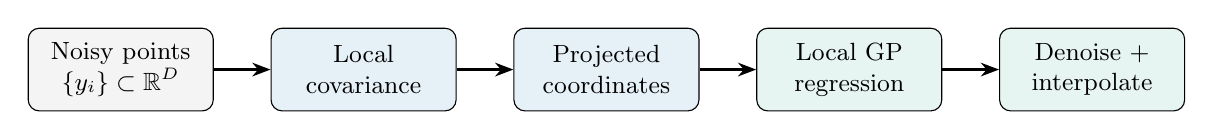
\begin{tikzpicture}[
      node distance=0.72cm,
      box/.style={draw, rounded corners, minimum width=2.35cm,
        minimum height=1.05cm, align=center, font=\small},
      arr/.style={-{Stealth}, thick}
    ]
      \node[box, fill=neutral!10] (data) {Noisy points\\\(\{y_i\}\subset\R^D\)};
      \node[box, fill=positive!10, right=of data] (cov) {Local\\covariance};
      \node[box, fill=positive!10, right=of cov] (coords) {Projected\\coordinates};
      \node[box, fill=emphasis!10, right=of coords] (gp) {Local GP\\regression};
      \node[box, fill=emphasis!10, right=of gp] (out) {Denoise +\\interpolate};
      \draw[arr] (data) -- (cov);
      \draw[arr] (cov) -- (coords);
      \draw[arr] (coords) -- (gp);
      \draw[arr] (gp) -- (out);
    \end{tikzpicture}
  \end{center}
  \vspace{0.25cm}
  \begin{alertblock}{Central reduction}
    A global manifold problem becomes many low-dimensional,
    errors-in-variables regressions.
  \end{alertblock}
\end{frame}

\section{Geometry to regression}

\begin{frame}{Local covariance}
  For a center \(y_k\), retain neighbors inside radius \(\epsilon\):
  \[
    C_{n,\epsilon}(y_k)=
    \frac1n\sum_{i=1}^n
    (y_i-y_k)(y_i-y_k)^\top
    \mathbf 1\{\|y_i-y_k\|\leq\epsilon\}.
  \]
  \begin{columns}[T]
    \column{0.54\textwidth}
      \begin{itemize}
        \item first \(d\) eigenvectors: high local variation
        \item remaining \(D-d\): normal directions
        \item no uniform-design assumption on \(P\)
      \end{itemize}
    \column{0.41\textwidth}
      \begin{center}
        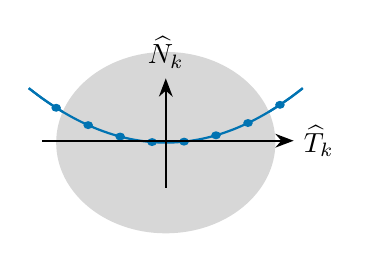
\begin{tikzpicture}[xscale=0.58,yscale=0.48]
          \draw[thick,positive] plot[smooth,domain=-3:3]
            (\x,{0.16*\x*\x});
          \fill[neutral!35] (0,0) circle (2.4cm);
          \draw[thick,positive] plot[smooth,domain=-3:3]
            (\x,{0.16*\x*\x});
          \foreach \x in {-2.4,-1.7,-1.0,-0.3,0.4,1.1,1.8,2.5} {
            \pgfmathsetmacro{\yy}{0.16*\x*\x}
            \fill[positive] (\x,\yy) circle (3pt);
          }
          \draw[-{Stealth},thick] (-2.7,0.05)--(2.8,0.05)
            node[right] {\(\widehat T_k\)};
          \draw[-{Stealth},thick] (0,-1.2)--(0,1.7)
            node[above] {\(\widehat N_k\)};
        \end{tikzpicture}
      \end{center}
  \end{columns}
\end{frame}

\begin{frame}{Local coordinates from eigendirections}
  Write
  \[
    C_{n,\epsilon}(y_k)
      =U_{n,\epsilon}(y_k)\Lambda_{n,\epsilon}(y_k)
       U_{n,\epsilon}(y_k)^\top .
  \]
  The rotation \(U_{n,\epsilon}(y_k)^\top\) defines two projections:
  \[
    \underbrace{P_{y_k}(y)}_{\R^D\to\R^d}
      =J^\top U_{n,\epsilon}(y_k)^\top(y-y_k),
    \qquad
    \underbrace{P^\perp_{y_k}(y)}_{\R^D\to\R^{D-d}}
      =\bar J^\top U_{n,\epsilon}(y_k)^\top(y-y_k).
  \]
  \begin{alertblock}{Roles}
    \(P_{y_k}(y)\): GP predictor;\quad
    \(P^\perp_{y_k}(y)\): multivariate GP response.
  \end{alertblock}
\end{frame}

\begin{frame}{Why a local graph is enough}
  Near a clean point \(y\in\iota(\M)\), rotate and translate the manifold:
  \[
    \Phi(u)=y+U
      \begin{bmatrix}u\\F(u)\end{bmatrix},
    \qquad F:\R^d\supset O\to\R^{D-d}.
  \]
  \begin{center}
    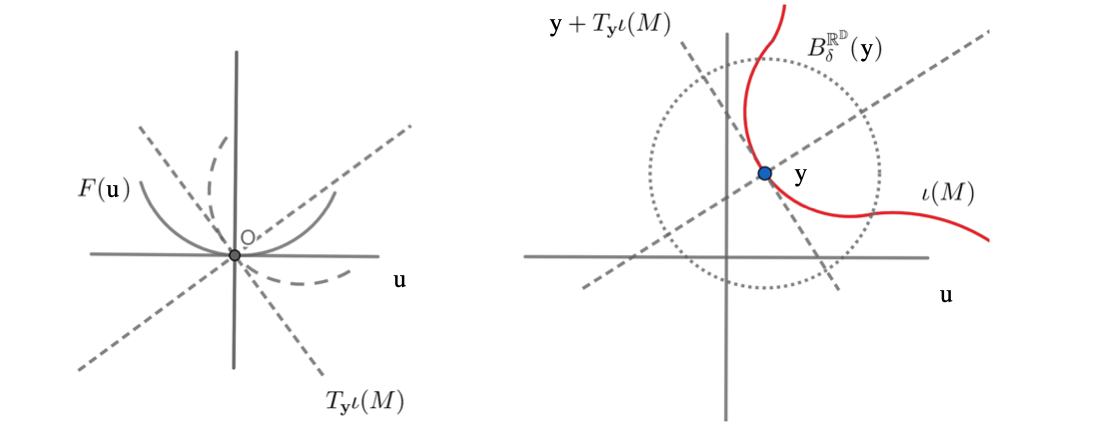
\includegraphics[width=0.72\textwidth]{figures/fig-local-graph.png}

    \footnotesize Source: Dunson and Wu (2026), Figure 2.
  \end{center}
\end{frame}

\begin{frame}{The key geometric relaxation}
  Classical local methods try to estimate the true tangent space
  \(T_{\iota(x_k)}\iota(\M)\).
  \vspace{0.2cm}
  \begin{columns}[T]
    \column{0.48\textwidth}
      \begin{block}{Stronger requirement}
        \[
          \widehat T_k\approx
          T_{\iota(x_k)}\iota(\M)
        \]
        Accurate tangent recovery at every sample.
      \end{block}
    \column{0.48\textwidth}
      \begin{exampleblock}{MrGap requirement}
        \[
          P_{y_k}\big|_{\iota(\M)}
          \text{ is locally invertible}
        \]
        Enough to write the manifold as a graph over \(H_k=y_k+\widehat T_k\).
      \end{exampleblock}
  \end{columns}
  \vspace{0.3cm}
  \centering
  \HL{Useful coordinates do not require a perfect tangent estimate.}
\end{frame}

\begin{frame}{Neighbors become regression pairs}
  For \(y_{k,j}\in B_\delta(y_k)\setminus\{y_k\}\), construct
  \[
    w_{k,j}=P_{y_k}(y_{k,j}),\qquad
    z_{k,j}=P^\perp_{y_k}(y_{k,j}).
  \]
  \begin{center}
    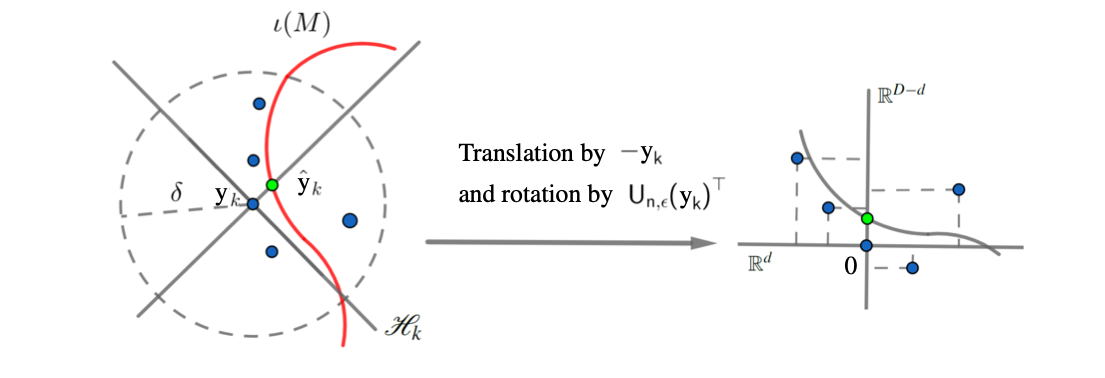
\includegraphics[width=0.75\textwidth]{figures/fig-denoising-transform.png}

    \footnotesize Source: Dunson and Wu (2026), Figure 3.
  \end{center}
\end{frame}

\begin{frame}{Local Gaussian process}
  The projected pairs obey an errors-in-variables representation:
  \[
    w_i=u_i+\eta_{i,1},\qquad
    z_i=F(u_i)+\eta_{i,2}.
  \]
  Independently for \(r=1,\ldots,D-d\),
  \[
    f_r\sim\operatorname{GP}(0,C),\qquad
    C(u,u')=A\exp\!\left\{-\frac{\|u-u'\|^2}{\rho}\right\}.
  \]
  \begin{columns}[T]
    \column{0.48\textwidth}
      \begin{itemize}
        \item shared \(A,\rho,\sigma\) across local fits
        \item empirical Bayes via summed marginal likelihood
      \end{itemize}
    \column{0.48\textwidth}
      \begin{itemize}
        \item prediction at \(u=0\): denoising
        \item prediction at new \(u\): interpolation
      \end{itemize}
  \end{columns}
\end{frame}

\begin{frame}{Where should $A$, $\rho$, and $\sigma$ come from?}
  MrGap shares one hyperparameter triple across all local regressions in round $t$:
  \[
    (\widehat A^{(t)},\widehat\rho^{(t)},\widehat\sigma^{(t)})
      =\arg\max_{A,\rho,\sigma}
        \sum_{k=1}^{n}\log p(Z_k\mid A,\rho,\sigma).
  \]
  \begin{center}
    \small
    \begin{tabular}{p{0.20\textwidth}p{0.68\textwidth}}
      \toprule
      Layer & What is available\\
      \midrule
      paper & summed marginal-likelihood objective; re-estimate each round\\
      public \texttt{Mfit1.m} & denoising conditional on supplied $A,\rho,\mathrm{sig}$; no optimizer\\
      %current benchmark & stored example-specific tuples; no per-round MLE\\
      \bottomrule
    \end{tabular}
  \end{center}
\end{frame}

\begin{frame}{Hyperparameters fixed in the current iteration scan}
  \begin{center}
    \small
    \begin{tabular}{lp{0.25\textwidth}p{0.25\textwidth}p{0.20\textwidth}}
      \toprule
      Manifold & round 1 $(A,\rho,\sigma^2)$ & rounds 2--5 $(A,\rho,\sigma^2)$ & provenance\\
      \midrule
      Cassini & $(.014,.2,.002)$ & $(.048,.3,2\!\times\!10^{-5})$ & paper \S4.1\\
      $\mathbb{RP}^{3}$ & $(.05,1,.0015)$ & $(.08,1.2,.0004)$ & reproduction setting\\
      Torus & $(.06,.2,.03)$ & $(.2,1.1,.007)$ & paper \S4.2\\
      Half-torus & $(1.3,5,.002)$ & $(1.3,5,.002)$ & reproduction setting\\
      \bottomrule
    \end{tabular}
  \end{center}
  \vspace{0.35cm}
\end{frame}

\section{Algorithm}

\begin{frame}{Why is the algorithm built from local pieces?}
  \begin{center}
    \small
    \begin{tabular}{p{0.30\textwidth}p{0.25\textwidth}p{0.34\textwidth}}
      \toprule
      Geometric obstacle & Design choice & What it buys\\
      \midrule
      no single global chart & overlapping patches & topology and changing axes\\
      unknown local orientation & covariance eigenspaces & tangent/normal coordinates\\
      manifold is curved & graph $F:\R^d\to\R^{D-d}$ & intrinsic-dimension regression\\
      observations are noisy & GP posterior mean & smooth correction and uncertainty\\
      frames improve after cleaning & repeat all local steps & updated neighbors, frames, fits\\
      \bottomrule
    \end{tabular}
  \end{center}
  \vspace{0.25cm}
  \centering
  \HL{Each component removes one obstruction to turning an unknown manifold into a regression problem.}
\end{frame}

\begin{frame}{Why predict only the normal displacement?}
  In an estimated local frame, a neighbor decomposes as
  \[
    y_j-y_k
      =\widehat T_k w_{k,j}+\widehat N_k z_{k,j},
    \qquad z_{k,j}\approx F_k(w_{k,j})+\text{noise}.
  \]
  The manifold point above the chart origin is therefore estimated by
  \[
    \widehat y_k=y_k+\widehat N_k\widehat F_k(0).
  \]
  \begin{columns}[T]
    \column{0.48\textwidth}
      \begin{block}{Keep the tangential coordinate fixed}
        Tangential motion changes location along the manifold; it does not
        identify the off-manifold error.
      \end{block}
    \column{0.48\textwidth}
      \begin{exampleblock}{Learn the normal graph}
        GP averaging estimates curvature while shrinking noisy normal residuals;
        posterior covariance quantifies local uncertainty.
      \end{exampleblock}
  \end{columns}
\end{frame}

\begin{frame}{Denoising phase}
  \begin{center}
    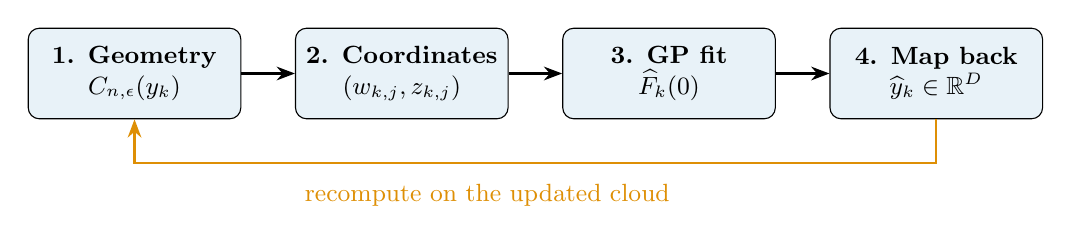
\begin{tikzpicture}[
      node distance=0.68cm,
      algostep/.style={draw, rounded corners, fill=positive!9,
        minimum width=2.7cm, minimum height=1.15cm,
        align=center, font=\small},
      arr/.style={-{Stealth}, thick}
    ]
      \node[algostep] (s1) {\textbf{1. Geometry}\\\(C_{n,\epsilon}(y_k)\)};
      \node[algostep, right=of s1] (s2) {\textbf{2. Coordinates}\\\((w_{k,j},z_{k,j})\)};
      \node[algostep, right=of s2] (s3) {\textbf{3. GP fit}\\\(\widehat F_k(0)\)};
      \node[algostep, right=of s3] (s4) {\textbf{4. Map back}\\\(\widehat y_k\in\R^D\)};
      \draw[arr] (s1)--(s2);
      \draw[arr] (s2)--(s3);
      \draw[arr] (s3)--(s4);
      \draw[arr,negative] (s4.south) -- ++(0,-0.55)
        -| node[pos=0.28,below=4pt,font=\small] {recompute on the updated cloud}
        (s1.south);
    \end{tikzpicture}
  \end{center}
  \vspace{0.25cm}
  \begin{alertblock}{Inputs and output}
    Inputs: \(\{y_i\},d,\epsilon,\delta\).\quad
    Output: \(\{\widehat y_i\}\) plus local predictive covariances.
  \end{alertblock}
\end{frame}

\begin{frame}{Prediction in the normal affine space}
  Partition the GP covariance over training predictors and \(0\):
  \[
    \Sigma_k=
    \begin{bmatrix}
      \Sigma_{k,1}&\Sigma_{k,2}\\
      \Sigma_{k,3}&\Sigma_{k,4}
    \end{bmatrix}.
  \]
  The local posterior mean maps back as
  \[
    \widehat y_k
      =y_k+U_{n,\epsilon}(y_k)
      \begin{bmatrix}
        0\\
        \{\Sigma_{k,3}(\Sigma_{k,1}+\sigma^2I)^{-1}Z_k\}^{\!\top}
      \end{bmatrix}.
  \]
  \begin{alertblock}{Geometric interpretation}
    Tangential coordinate fixed at \(0\); correction occurs in the estimated
    normal affine space \(A_k=y_k+\widehat N_k\).
  \end{alertblock}
\end{frame}

\begin{frame}{Why iterate the denoising map?}
  \begin{center}
    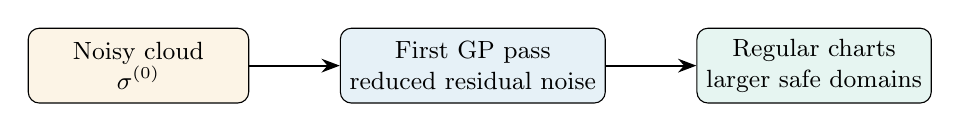
\begin{tikzpicture}[
      node distance=1.15cm,
      state/.style={draw, rounded corners, minimum width=2.8cm,
        minimum height=0.95cm, align=center, font=\small},
      arr/.style={-{Stealth},thick}
    ]
      \node[state,fill=negative!10] (a) {Noisy cloud\\\(\sigma^{(0)}\)};
      \node[state,fill=positive!10,right=of a] (b) {First GP pass\\reduced residual noise};
      \node[state,fill=emphasis!10,right=of b] (c) {Regular charts\\larger safe domains};
      \draw[arr] (a)--(b);
      \draw[arr] (b)--(c);
    \end{tikzpicture}
  \end{center}
  \vspace{0.35cm}
  \begin{itemize}
    \item the first correction changes distances and neighborhood membership
    \item reduced normal noise can sharpen the next local PCA frame
    \item the next GP is fitted in updated coordinates, not merely reapplied
  \end{itemize}
  \begin{alertblock}{Stopping is part of the estimator}
    Paper: stop when $|\widehat\sigma^{(t)}-\widehat\sigma^{(t-1)}|$ is small.
    Current fixed-parameter scan: this criterion is not evaluated.
  \end{alertblock}
\end{frame}

\begin{frame}{Interpolation has two extra challenges}
  Given a local chart, a new point would be
  \[
    \widetilde y_{k,j}
      =y_k+U_{n,\epsilon}(y_k)
        \begin{bmatrix}
          \widetilde u_{k,j}\\
          \widehat F_k(\widetilde u_{k,j})
        \end{bmatrix}.
  \]
  \begin{columns}[T]
    \column{0.48\textwidth}
      \begin{block}{Unknown domain}
        \(\widetilde u_{k,j}\) must remain inside the unknown chart domain \(O_k\).
      \end{block}
    \column{0.48\textwidth}
      \begin{block}{Chart seams}
        Independent predictions from overlapping charts can leave visible gaps.
      \end{block}
  \end{columns}
\end{frame}

\begin{frame}{Sequential interpolation stitches local charts}
  When processing chart \(k\), reuse earlier interpolations that fall inside
  \(B_\delta(y_k)\) as additional regression pairs.
  \begin{center}
    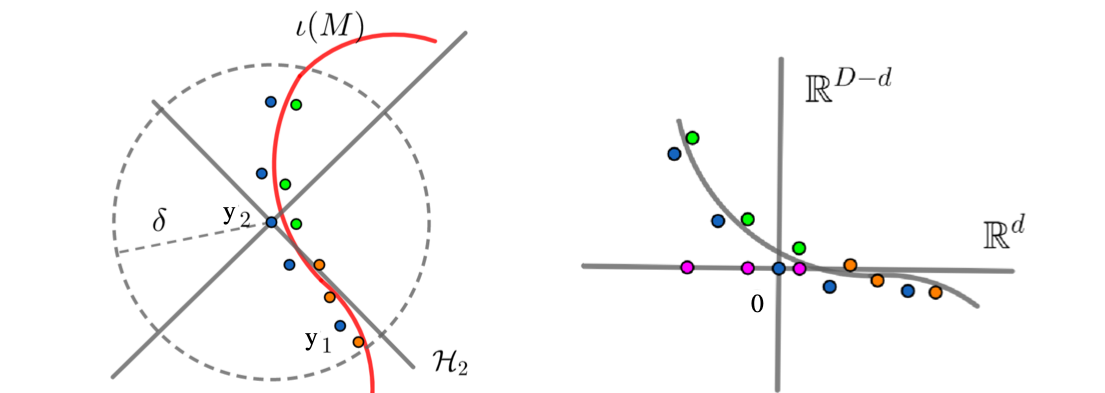
\includegraphics[width=0.75\textwidth]{figures/fig-sequential-interpolation.png}

    \footnotesize Source: Dunson and Wu (2026), Figure 4.
  \end{center}
  \vspace{-0.1cm}
  \centering
  \HL{Overlap information couples otherwise independent local GPs.}
\end{frame}

\begin{frame}{Choosing the geometric scales}
  \begin{center}
    \begin{tabular}{lll}
      \toprule
      Parameter & Geometric role & Statistical trade-off\\
      \midrule
      \(\epsilon\) & covariance neighborhood
        & eigenspace variance vs.\ curvature bias\\
      \(\delta\) & regression neighborhood
        & sample size vs.\ chart validity\\
      \(\rho\) & GP correlation length
        & local flexibility vs.\ smoothness\\
      \(\sigma\) & noise scale
        & shrinkage toward the fitted graph\\
      \bottomrule
    \end{tabular}
  \end{center}
  \vspace{0.25cm}
  \begin{alertblock}{Paper's strategy}
    Grid search over \(\epsilon\leq\delta\); optimize
    \(A,\rho,\sigma\) by the summed local marginal likelihood.
  \end{alertblock}
\end{frame}

\section{Theory}

\begin{frame}{Theory roadmap}
  \begin{center}
    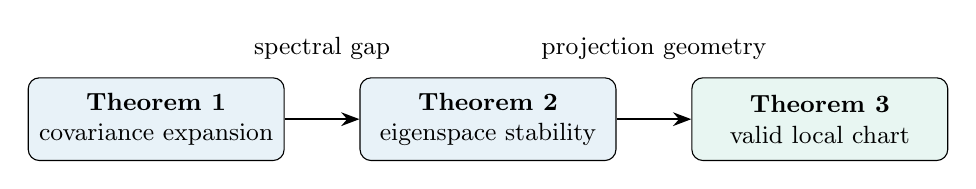
\begin{tikzpicture}[
      node distance=0.95cm,
      thm/.style={draw,rounded corners,minimum width=3.25cm,
        minimum height=1.05cm,align=center,font=\small},
      arr/.style={-{Stealth},thick}
    ]
      \node[thm,fill=positive!9] (t1) {\textbf{Theorem 1}\\covariance expansion};
      \node[thm,fill=positive!9,right=of t1] (t2) {\textbf{Theorem 2}\\eigenspace stability};
      \node[thm,fill=emphasis!9,right=of t2] (t3) {\textbf{Theorem 3}\\valid local chart};
      \draw[arr] (t1)--node[above=18pt,font=\small]{spectral gap}(t2);
      \draw[arr] (t2)--node[above=18pt,font=\small]{projection geometry}(t3);
    \end{tikzpicture}
  \end{center}
  \vspace{0.35cm}
  \begin{exampleblock}{Operational conclusion}
    With compatible \(n,\epsilon,\delta,\sigma\), the projected data genuinely
    support a local regression representation of the manifold.
  \end{exampleblock}
\end{frame}

\begin{frame}{Theorem 1: covariance separates directions}
  After centering and rotating so that the first \(d\) axes are tangent,
  \[
    C_{n,\epsilon}(y_k)
      =
      \epsilon^{d+2}
      \frac{|S^{d-1}|P(x_k)}{d(d+2)}
      \begin{bmatrix}I_d&0\\0&0\end{bmatrix}
      +E_{n,\epsilon,\sigma}.
  \]
  \begin{columns}[T]
    \column{0.48\textwidth}
      \begin{itemize}
        \item signal occupies a rank-\(d\) block
        \item density \(P(x_k)\) changes scale, not directions
      \end{itemize}
    \column{0.48\textwidth}
      \begin{itemize}
        \item curvature, finite \(n\), noise enter through \(E\)
        \item small \(E\) yields a local spectral gap
      \end{itemize}
  \end{columns}
  \begin{alertblock}{Implication}
    Local PCA remains informative under nonuniform sampling and Gaussian noise.
  \end{alertblock}
\end{frame}

\begin{frame}{Theorem 2: eigenspaces are stable enough}
  Davis--Kahan perturbation control gives
  \[
    U_{n,\epsilon}(y_k)
      =
      \begin{bmatrix}X_1&0\\0&X_2\end{bmatrix}
      +O\!\left(\epsilon^{2\min(\beta-1,1)}\right),
  \]
  where \(X_1\in O(d)\), \(X_2\in O(D-d)\).
  \begin{columns}[T]
    \column{0.48\textwidth}
      \begin{block}{What is identified}
        Tangent and normal \emph{subspaces}, up to rotations within each.
      \end{block}
    \column{0.48\textwidth}
      \begin{exampleblock}{What the algorithm needs}
        A coordinate projection that preserves local one-to-one geometry.
      \end{exampleblock}
  \end{columns}
\end{frame}

\begin{frame}{Theorem 3: projection really defines a chart}
  For \(\epsilon^\beta<\delta<\tau_{\iota(\M)}/16\), with high probability:
  \begin{enumerate}
    \item noisy neighbors in \(B_\delta(y_k)\) originate from the larger clean neighborhood;
    \item \(P_{y_k}\) is a diffeomorphism on
      \(B_{3\delta}(y_k)\cap\iota(\M)\);
    \item the image \(O_k\subset\R^d\) contains \(0\) and a nontrivial round ball.
  \end{enumerate}
  \begin{alertblock}{Why this is the pivotal result}
    It justifies \(F_k=P^\perp_{y_k}\circ P_{y_k}^{-1}\), turning manifold
    reconstruction into regression without observing tangent spaces.
  \end{alertblock}
\end{frame}

\begin{frame}{Reading the assumptions statistically}
  \vspace{4pt}
  \begin{center}
    \begin{tabular}{p{0.25\textwidth}p{0.30\textwidth}p{0.34\textwidth}}
      \toprule
      Assumption & Why it appears & Practical warning\\
      \midrule
      smooth closed \(\M\) & uniform local charts & boundaries need modification\\
      positive smooth \(P\) & enough neighbors everywhere & sparse regions unstable\\
      isotropic Gaussian noise & rotation preserves noise law & anisotropy can bias coordinates\\
      small \(\epsilon\) vs.\ reach & avoid chart folding & high curvature narrows locality\\
      large \(n\) vs.\ \(\epsilon^{-d}\) & covariance concentration & intrinsic dimension matters\\
      \bottomrule
    \end{tabular}
  \end{center}
  \vspace{0.2cm}
  \centering
  \HL{The theory validates the reduction; it is not a full contraction-rate result for the GP estimator.}
\end{frame}

\section{Evidence}

\begin{frame}{Evidence in one dimension: Cassini oval}
  \begin{columns}[T]
    \column{0.62\textwidth}
      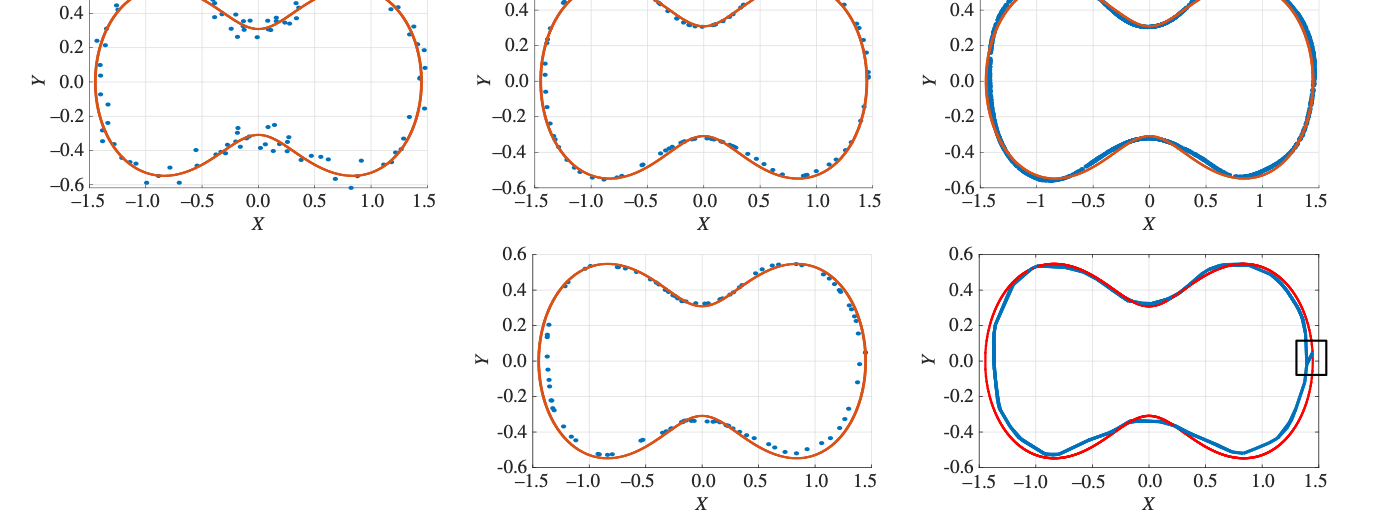
\includegraphics[width=\textwidth]{figures/fig-cassini-results.png}
    \column{0.34\textwidth}
      \vspace{0.25cm}
      \begin{center}
        \small
        \begin{tabular}{lr}
          \toprule
          Output & \(G\)\\
          \midrule
          noisy & 0.0590\\
          MrGap denoised & \textbf{0.0224}\\
          MrGap interp. & \textbf{0.0216}\\
          principal graph & 0.0322\\
          \bottomrule
        \end{tabular}
      \end{center}
      \vspace{0.2cm}
      Principal graph: visible nonsmooth seam.
  \end{columns}
  \vspace{0.05cm}
  \centering
  \footnotesize Source: Dunson and Wu (2026), Figure 6.
\end{frame}

\begin{frame}{Evidence in two dimensions: torus}
  \begin{columns}[T]
    \column{0.61\textwidth}
      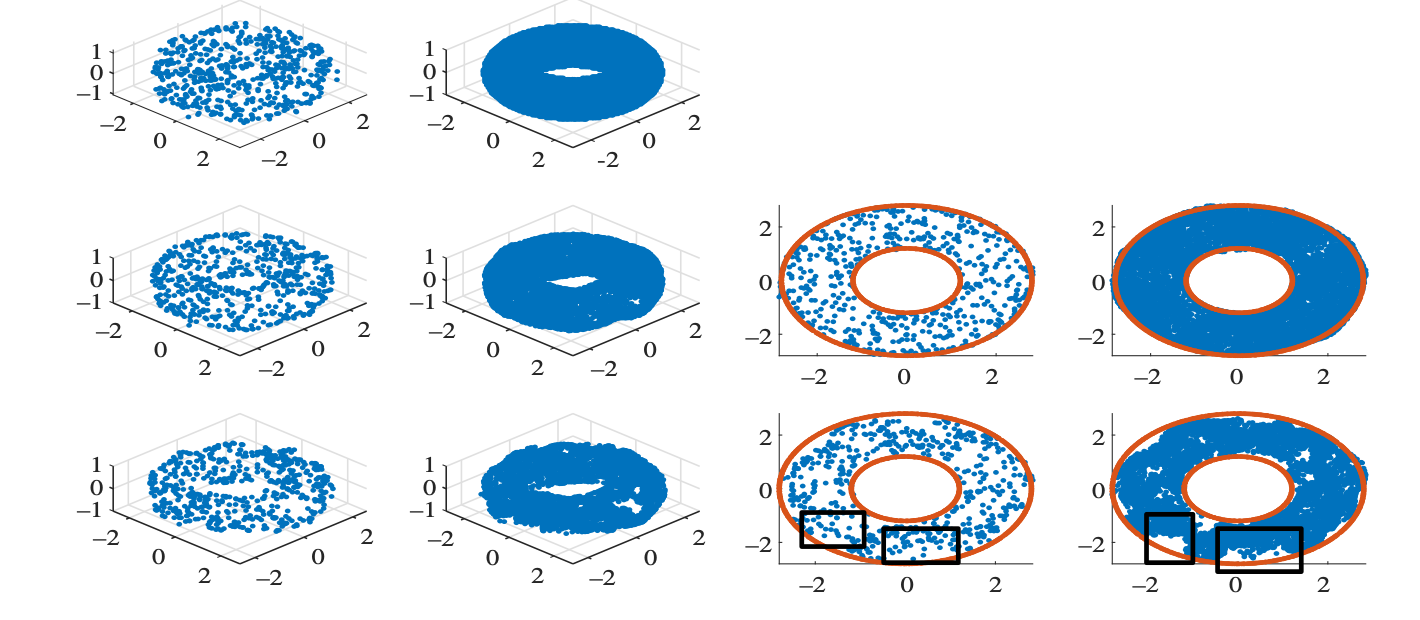
\includegraphics[width=\textwidth]{figures/fig-torus-results.png}
    \column{0.35\textwidth}
      \begin{center}
        \small
        \begin{tabular}{lr}
          \toprule
          Output & \(G\)\\
          \midrule
          noisy & 0.1238\\
          MrGap denoised & \textbf{0.0544}\\
          MrGap interp. & \textbf{0.0605}\\
          comparator den. & 0.2196\\
          comparator interp. & 0.2424\\
          \bottomrule
        \end{tabular}
      \end{center}
      \vspace{0.25cm}
      \HL{MrGap preserves the annular geometry}; the comparator shrinks the torus.
  \end{columns}
  \vspace{0.05cm}
  \centering
  \footnotesize Source: Dunson and Wu (2026), Figure 7.
\end{frame}

\section{Empirical benchmark}

\begin{frame}{Reproducing and benckmarks}
  \begin{center}
    \small
    \begin{tabular}{p{0.23\textwidth}p{0.67\textwidth}}
      \toprule
      Component & Pilot design\\
      \midrule
      Manifolds & Cassini oval, $\mathbb{RP}^{3}$, torus, half-torus\\
      Ambient noise & $\sigma\in\{0,.01,.02,.04,.06,.08,.12\}$\\
      Sample size & $n\in\{50,100,250,500,1000,5000\}$; fresh samples at every $n$\\
      Methods & MrGap after rounds 1--5; Manifold Fitting; oracle-tangent MrGap\\
      Diagnostics & geometric RMSE $G$, paired reconstruction RMSE, runtime, median local count $m_k$\\
      \bottomrule
    \end{tabular}
  \end{center}
\end{frame}

\begin{frame}{Pilot defaults}
  \begin{center}
    \small
    \begin{tabular}{lrrccrr}
      \toprule
      Manifold & $n$ & $\sigma$ & \multicolumn{2}{c}{$G$} & \multicolumn{2}{c}{runtime (s)}\\
      \cmidrule(lr){4-5}\cmidrule(lr){6-7}
       & & & MrGap--2 & MF & MrGap--2 & MF\\
      \midrule
      Cassini & 102 & .04 & \textbf{.0282} & .0285 & .023 & \textbf{.012}\\
      $\mathbb{RP}^{3}$ & 500 & .04 & .0886 & \textbf{.0797} & .129 & \textbf{.056}\\
      Torus & 500 & .12 & .0711 & \textbf{.0691} & .124 & \textbf{.056}\\
      Half-torus & 400 & .12 & \textbf{.0587} & .0670 & .100 & \textbf{.045}\\
      \bottomrule
    \end{tabular}
  \end{center}
  \vspace{0.25cm}
  \begin{columns}[T]
    \column{0.47\textwidth}
      \textbf{Accuracy:} ranking changes with geometry; neither method dominates.
    \column{0.47\textwidth}
      \textbf{Cost:} Manifold Fitting is about twice as fast at these small pilot sizes.
  \end{columns}
\end{frame}

\begin{frame}{Useful MrGap stopping points are two or three rounds}
  \centering
  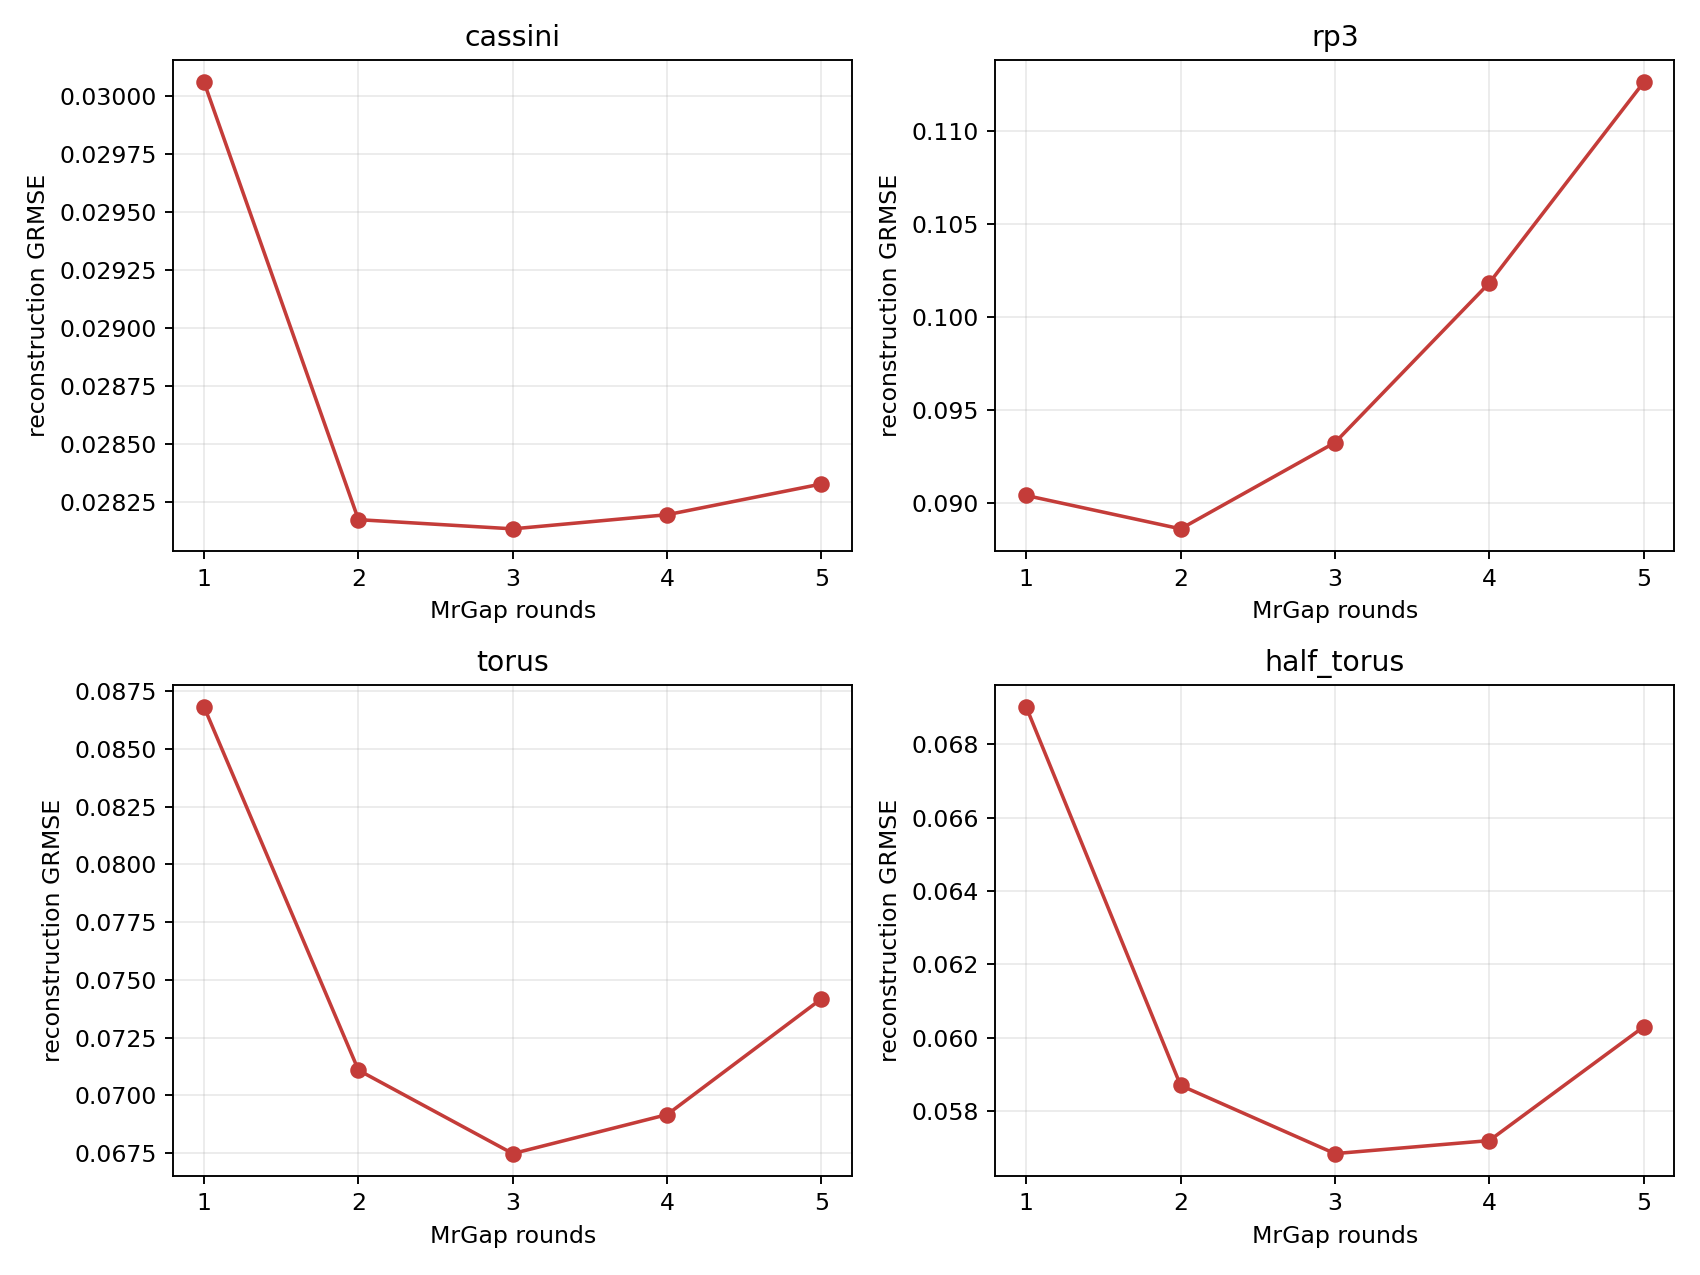
\includegraphics[width=0.80\textwidth,height=0.56\textheight,keepaspectratio]{figures/fig-benchmark-iterations.png}


  \vspace{0.08cm}
  \footnotesize Fixed-parameter diagnostic: round 1 uses the first tuple; rounds 2--5 reuse the final tuple. This is not an MLE convergence test.
\end{frame}

\begin{frame}{Noise sensitivity: failure is geometry-dependent}
  \centering
  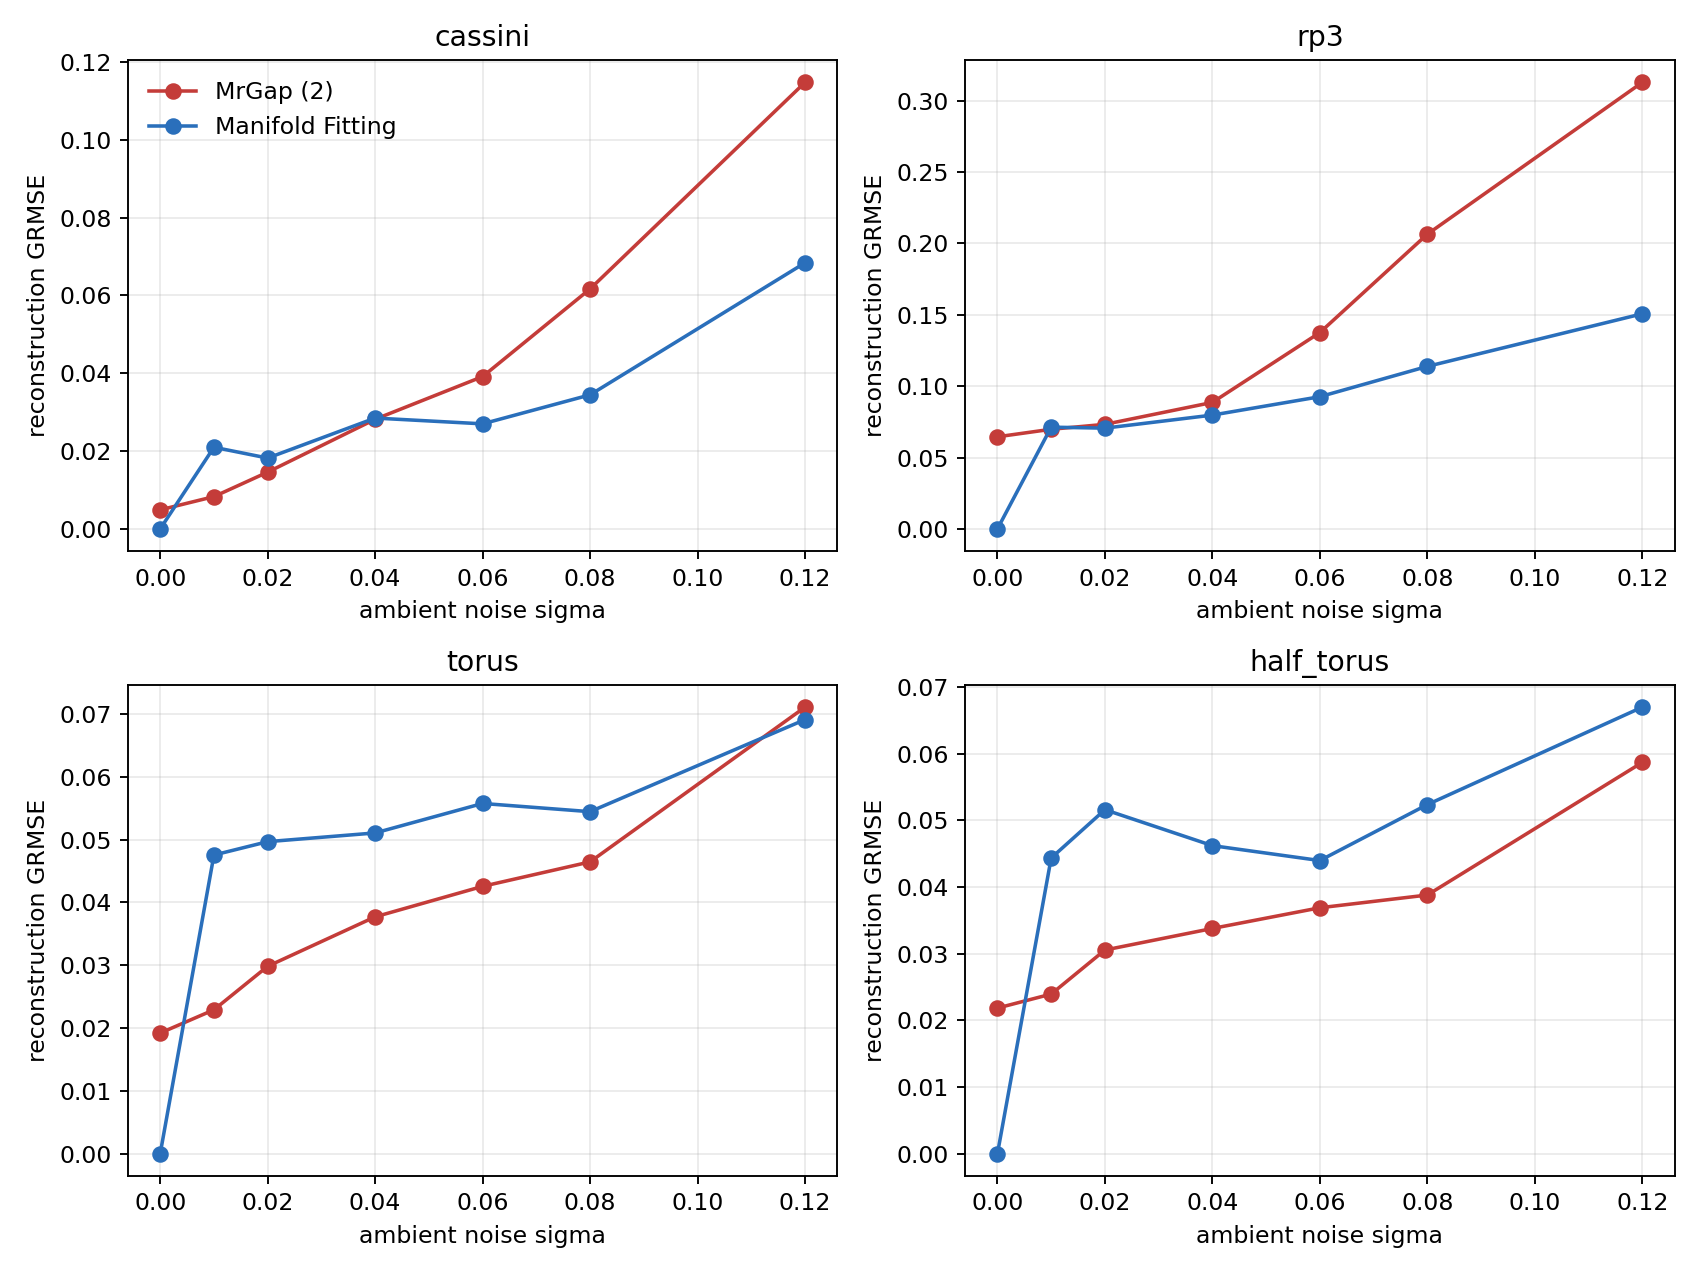
\includegraphics[width=0.82\textwidth,height=0.56\textheight,keepaspectratio]{figures/fig-benchmark-noise.png}

  \vspace{-0.05cm}
  \small
  The winner can change across the same
  noise grid, so a single Cassini setting is not representative.

  \vspace{0.08cm}
  \footnotesize MF uses the known noise level
\end{frame}

\begin{frame}{Global sample size: more data help only through local support}
  \centering
  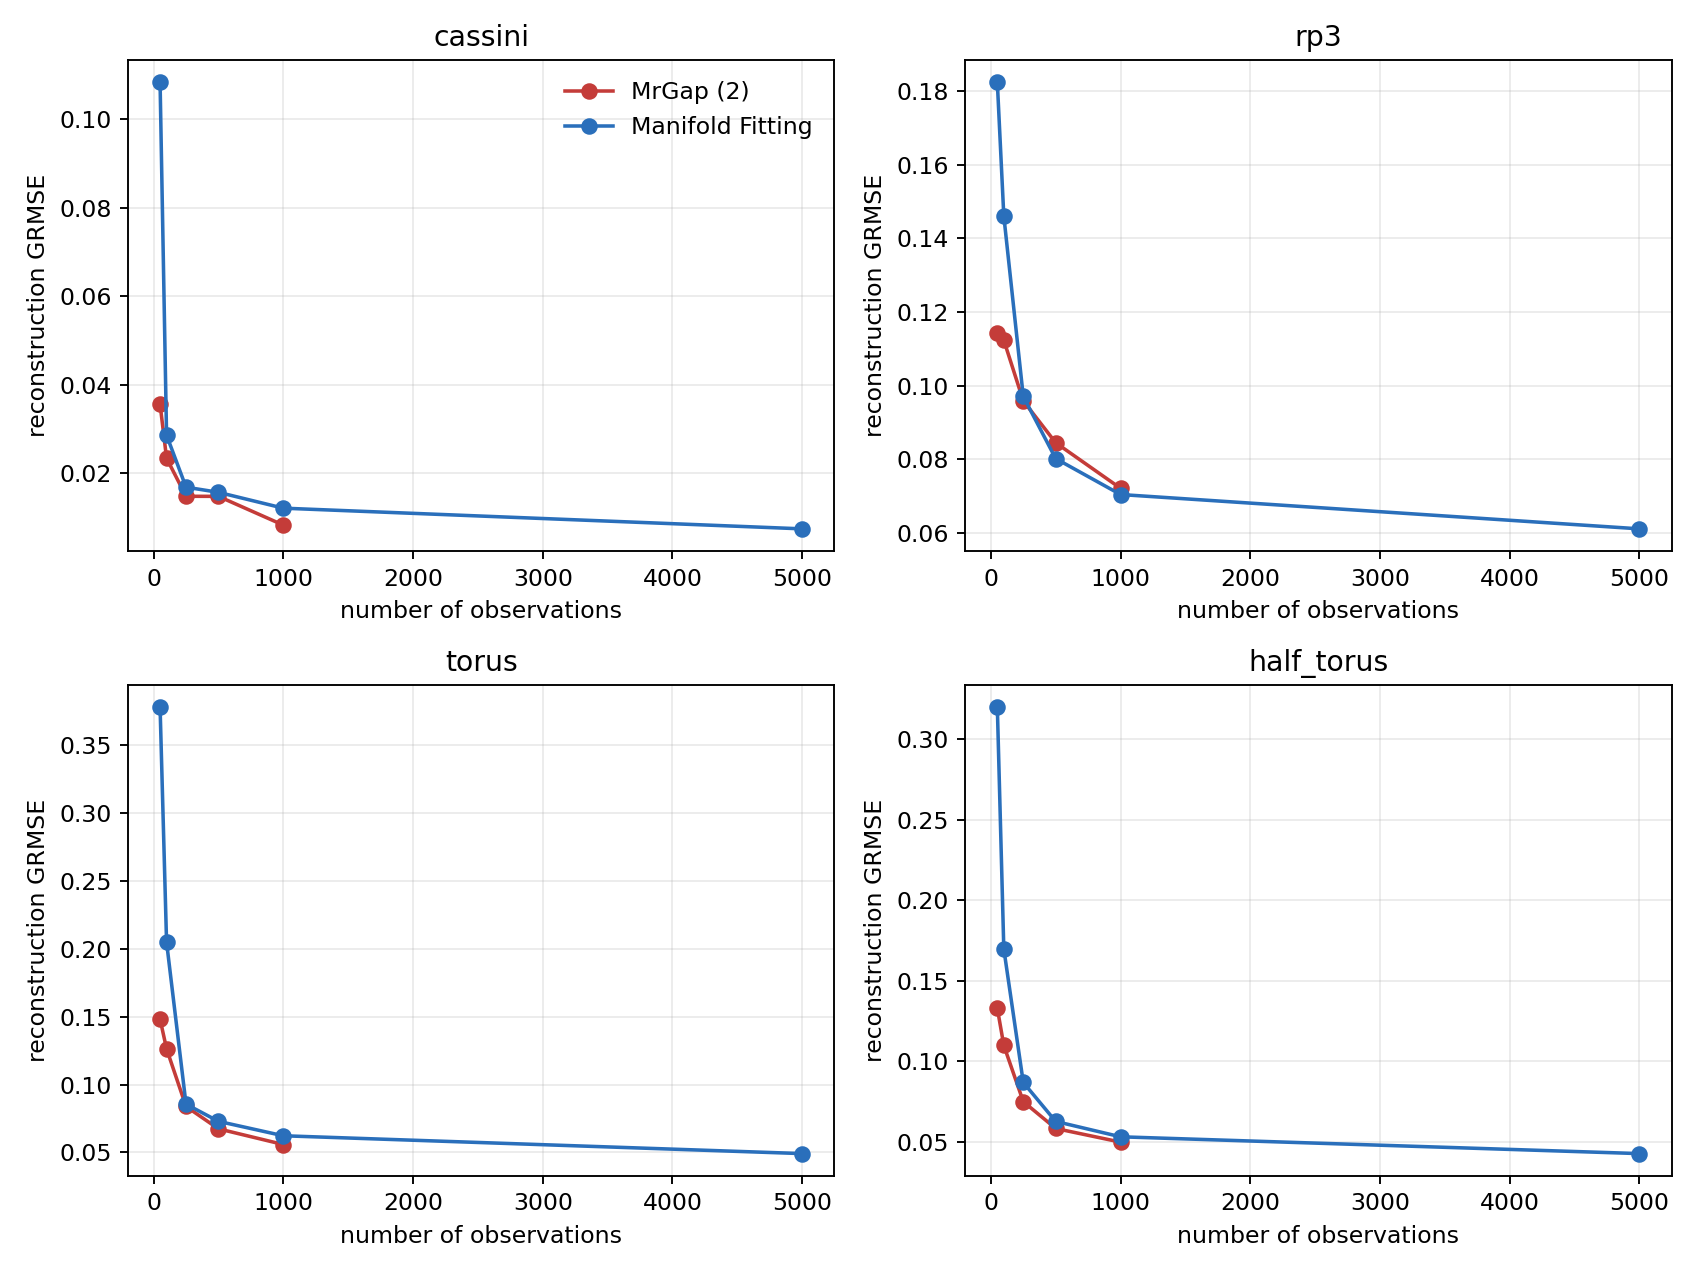
\includegraphics[width=0.82\textwidth,height=0.56\textheight,keepaspectratio]{figures/fig-benchmark-sample-size.png}

  \vspace{-0.05cm}
  \small
  Each $n$ is generated independently rather than subsampled from a fixed
  $100{,}000$-point cloud. Curves are nonmonotone when fixed neighborhoods
  trade variance for curvature bias.

  \vspace{0.08cm}
  \footnotesize Exact MrGap pilot runs stop at $n=1000$; $n=5000$ is omitted by the resource guard.
\end{frame}

\begin{frame}{Effective sample size is the local count $m_k$}
  \centering
  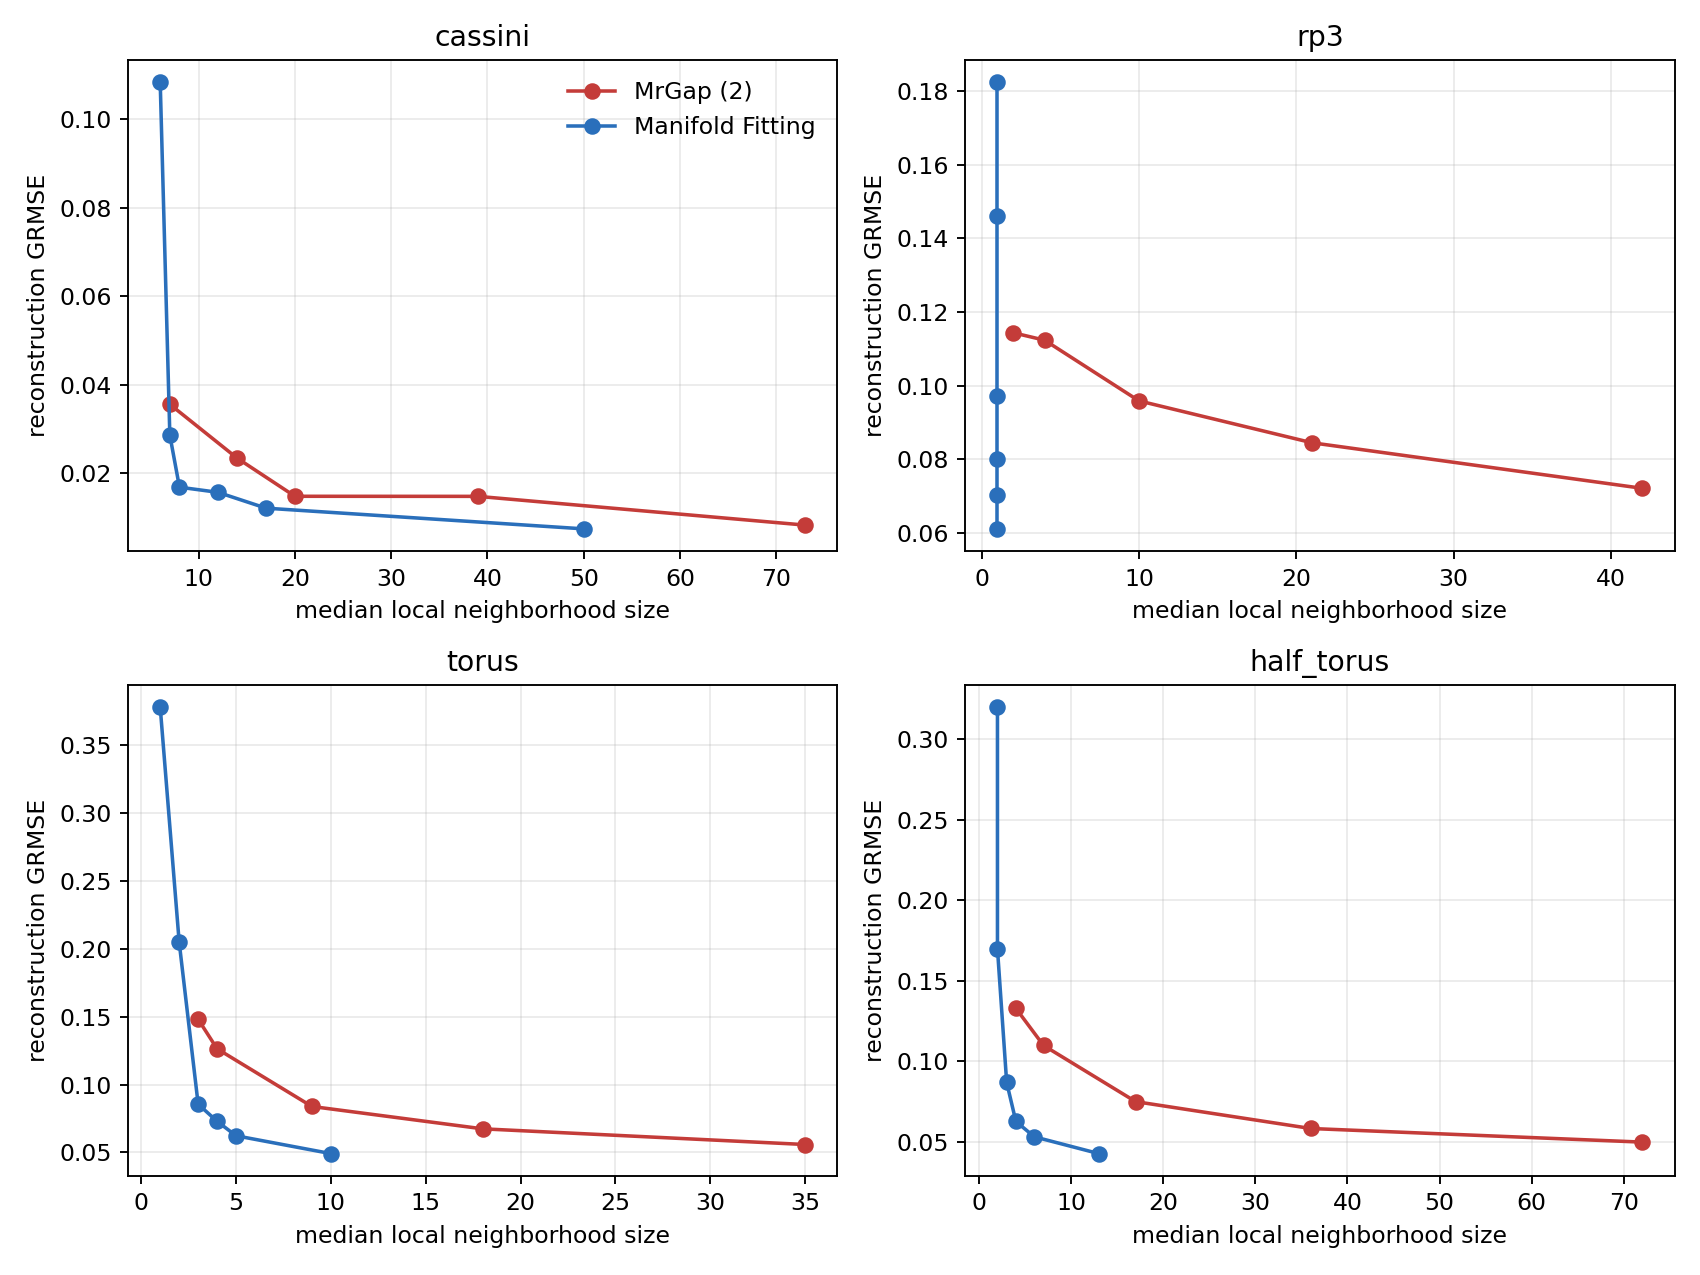
\includegraphics[width=0.82\textwidth,height=0.56\textheight,keepaspectratio]{figures/fig-benchmark-local-neighbors.png}

  \vspace{-0.05cm}
  \small
  Global $n$ is an incomplete predictor of error. On $\mathbb{RP}^{3}$,
  Manifold Fitting frequently reaches its official five-nearest-neighbor
  fallback because the cylindrical neighborhood is sparse.

  \vspace{0.08cm}
  \footnotesize Horizontal axis: median neighborhood size over reconstructed points.
\end{frame}

\begin{frame}{Bandwidth scan separates variance from curvature bias}
  \centering
  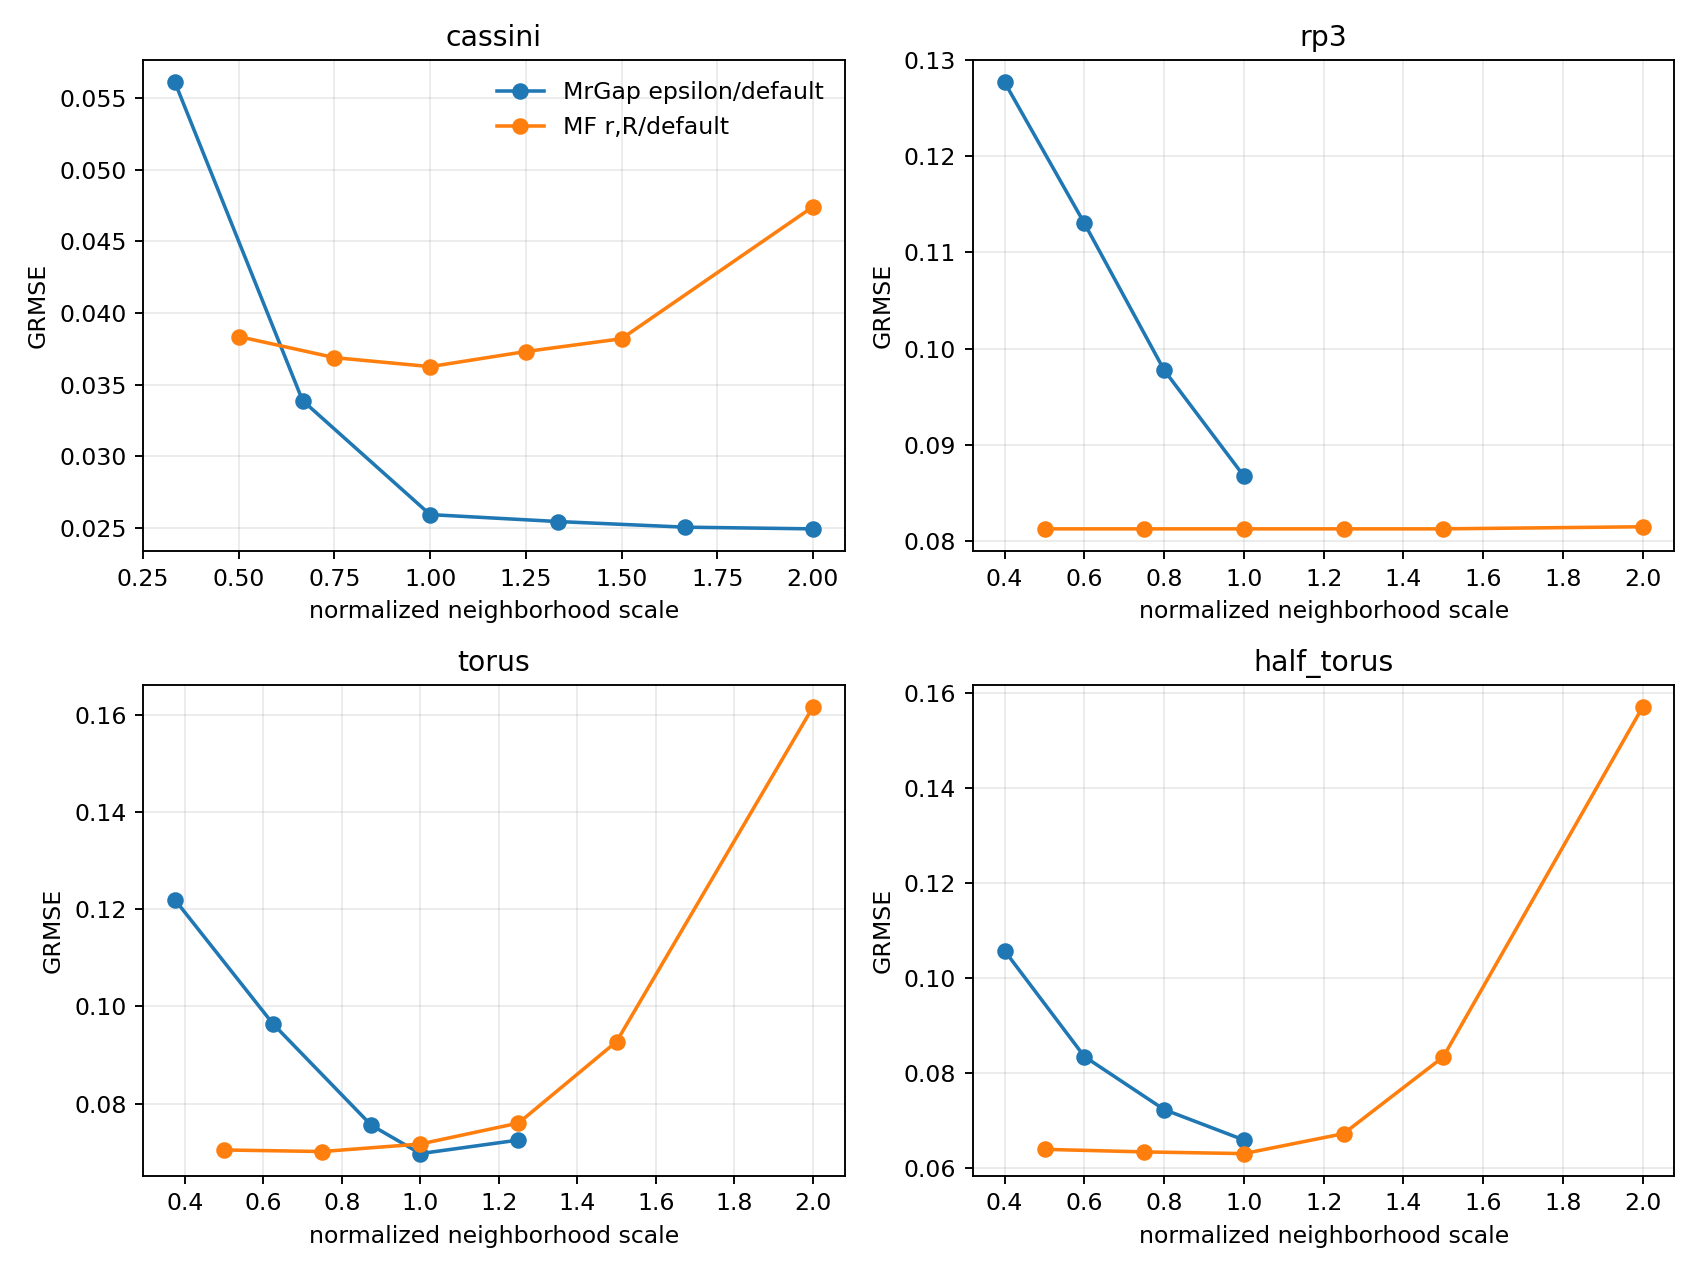
\includegraphics[width=0.82\textwidth,height=0.56\textheight,keepaspectratio]{figures/fig-benchmark-bandwidth.png}

  \vspace{-0.05cm}
  \small
  Too-small neighborhoods provide unstable local fits; too-large neighborhoods
  average across curvature. The pilot optima differ substantially by manifold.

  \vspace{0.08cm}
  \footnotesize MF horizontal axis rescales both official radii; MrGap horizontal axis is $\epsilon$.
\end{frame}

\begin{frame}{Oracle tangents isolate the chart-estimation bottleneck}
  \centering
  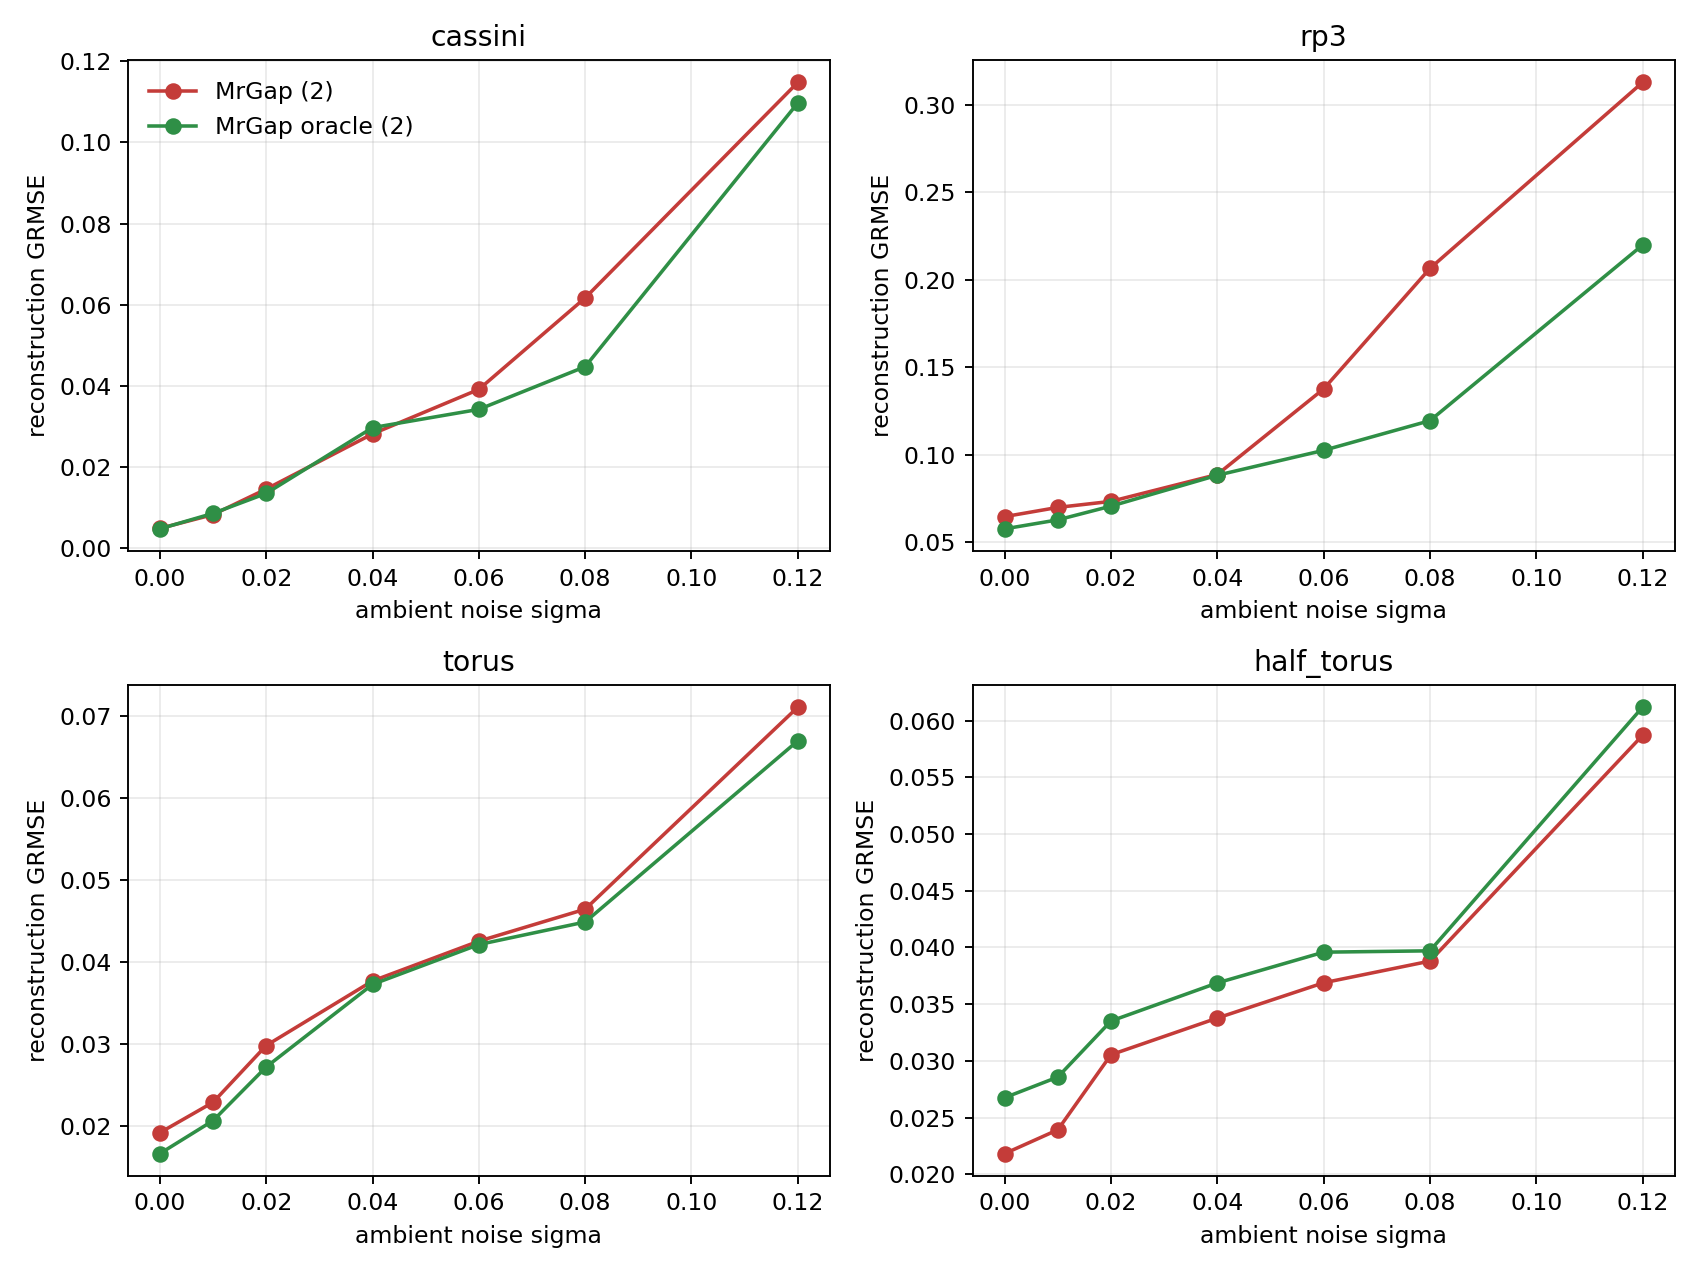
\includegraphics[width=0.82\textwidth,height=0.56\textheight,keepaspectratio]{figures/fig-benchmark-oracle.png}

  \vspace{-0.05cm}
  \small
  \footnotesize Oracle changes only the tangent basis; all other MrGap settings are fixed.
\end{frame}

\begin{frame}{Runtime scaling: the current implementations target different regimes}
  \centering
  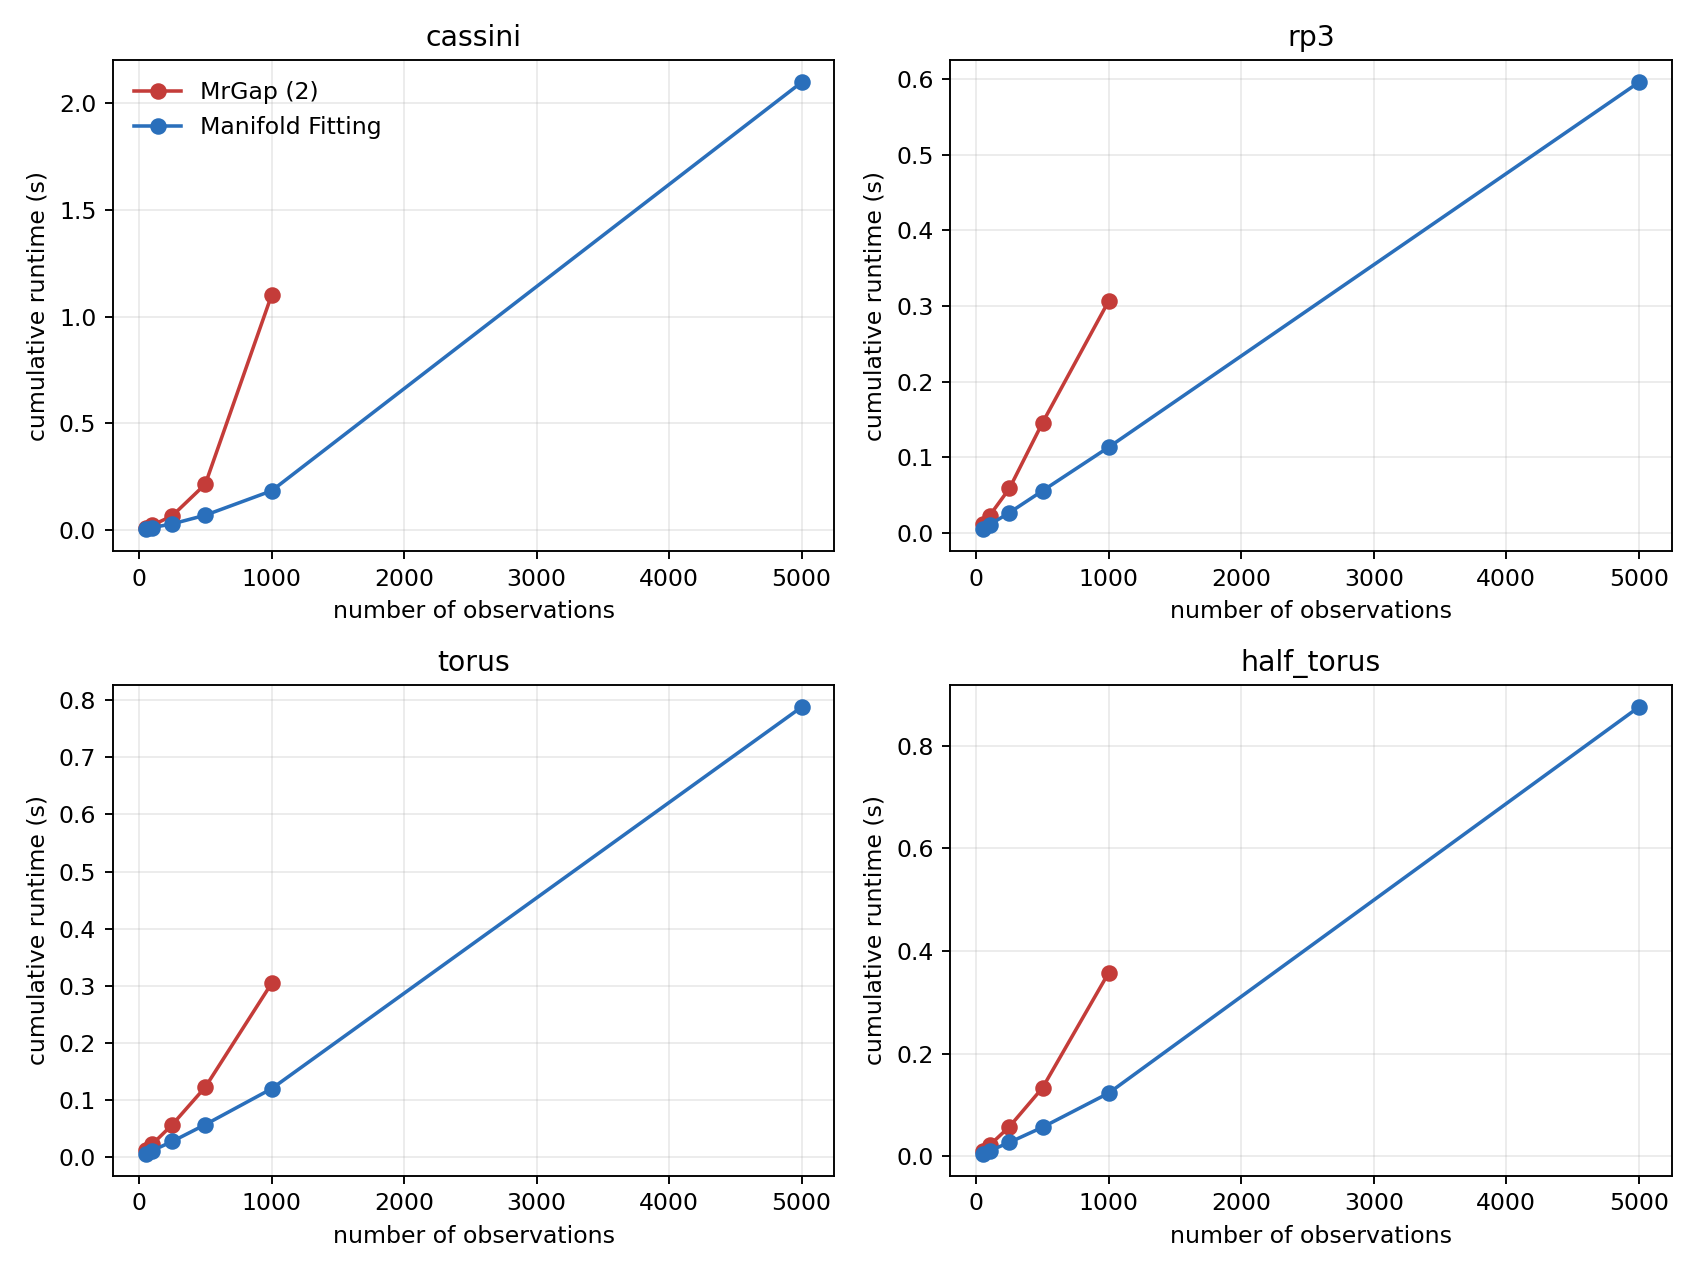
\includegraphics[width=0.82\textwidth,height=0.56\textheight,keepaspectratio]{figures/fig-benchmark-runtime.png}

  \vspace{-0.05cm}
  \small
  Manifold Fitting is faster throughout the pilot.

  \vspace{0.08cm}
\end{frame}

\section{Discussion: coupled local GPs}

\begin{frame}{Why couple neighboring local GPs?}
  Independent charts describe the \emph{same physical manifold} on overlaps:
  \[
    \Phi_k(u)=y_k+T_ku+N_kF_k(u)
    =
    y_\ell+T_\ell v+N_\ell F_\ell(v)=\Phi_\ell(v).
  \]
  \begin{columns}[T]
    \column{0.48\textwidth}
      \begin{block}{Independent MrGap fits}
        \[
          F_k\ \perp\!\!\!\perp\ F_\ell
        \]
        Agreement encouraged only through sequentially reused interpolations.
      \end{block}
    \column{0.48\textwidth}
      \begin{exampleblock}{Proposed coupled model}
        \[
          \operatorname{Cov}\{F_k(u),F_\ell(v)\}\neq0
        \]
        Share information in sparse regions; reduce seams across charts.
      \end{exampleblock}
  \end{columns}
  \vspace{0.2cm}
  \centering
  \HL{The meaningful constraint is ambient agreement of \(\Phi_k\) and \(\Phi_\ell\), not equality of raw GP coordinates.}
\end{frame}

\begin{frame}{Why a naive cross-chart covariance is ill-defined}
  On \(U_k\cap U_\ell\), four identifications are required:
  \vspace{0.15cm}
  \begin{center}
    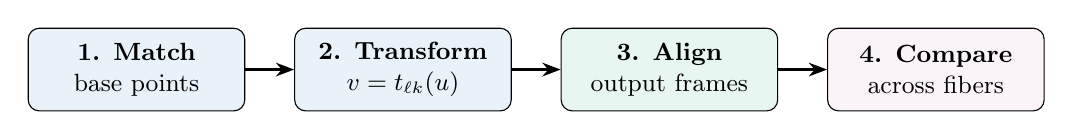
\begin{tikzpicture}[
      node distance=0.62cm,
      box/.style={draw,rounded corners,minimum width=2.75cm,
        minimum height=1.05cm,align=center,font=\small},
      arr/.style={-{Stealth},thick}
    ]
      \node[box,fill=positive!9] (match) {\textbf{1. Match}\\base points};
      \node[box,fill=positive!9,right=of match] (input) {\textbf{2. Transform}\\\(v=t_{\ell k}(u)\)};
      \node[box,fill=emphasis!9,right=of input] (frame) {\textbf{3. Align}\\output frames};
      \node[box,fill=cbPurple!9,right=of frame] (transport) {\textbf{4. Compare}\\across fibers};
      \draw[arr] (match)--(input);
      \draw[arr] (input)--(frame);
      \draw[arr] (frame)--(transport);
    \end{tikzpicture}
  \end{center}
  \begin{alertblock}{Normal-bundle caveat}
    \(N_kF_k(u)\in\operatorname{span}(N_k)\), a fixed transverse space;
    generally \(N_kF_k(u)\notin N_{\Phi_k(u)}\M\).
  \end{alertblock}
  \centering
  Frame alignment alone is insufficient: both the input transition and output
  identification vary over the overlap.
\end{frame}

\begin{frame}{A defensible coupled-GP construction}
  \begin{center}
    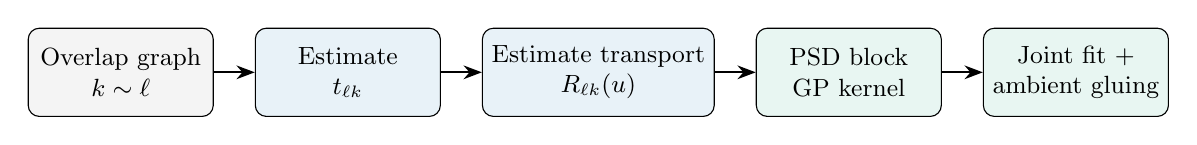
\begin{tikzpicture}[
      node distance=0.52cm,
      box/.style={draw,rounded corners,minimum width=2.35cm,
        minimum height=1.12cm,align=center,font=\small},
      arr/.style={-{Stealth},thick}
    ]
      \node[box,fill=neutral!10] (graph) {Overlap graph\\\(k\sim\ell\)};
      \node[box,fill=positive!9,right=of graph] (trans) {Estimate\\\(t_{\ell k}\)};
      \node[box,fill=positive!9,right=of trans] (align) {Estimate transport\\\(R_{\ell k}(u)\)};
      \node[box,fill=emphasis!9,right=of align] (kernel) {PSD block\\GP kernel};
      \node[box,fill=emphasis!9,right=of kernel] (fit) {Joint fit +\\ambient gluing};
      \draw[arr] (graph)--(trans);
      \draw[arr] (trans)--(align);
      \draw[arr] (align)--(kernel);
      \draw[arr] (kernel)--(fit);
    \end{tikzpicture}
  \end{center}
  A schematic cross-covariance is
  \[
    K_{k\ell}(u,v)
      =\kappa\!\left\{\dist_{\mathrm{graph}}(u,v)\right\}
       R_{k\ell}(u,v),\qquad v\approx t_{\ell k}(u).
  \]
  \begin{itemize}
    \item connection-Laplacian methods: data-driven frame transport
    \item gauge-independent projected kernels: valid covariance under frame changes
    \item alternate geometry estimation and joint GP fitting
  \end{itemize}
\end{frame}

\begin{frame}{Coupling does not remove measurement-error bias}
  The local regression is errors-in-variables:
  \[
    W=U+\xi,\qquad Z=F(U)+\zeta.
  \]
  A standard GP fitted to \((W,Z)\) targets
  \[
    m_\sigma(w)=\mathbb E(Z\mid W=w)
      =\frac{\{Fp\}*\varphi_\sigma(w)}
             {p*\varphi_\sigma(w)},
  \]
  not \(F(w)\) when predictor noise is nonnegligible.
  \begin{alertblock}{Required error decomposition}
    Chart/frame estimation \(+\) measurement-error bias \(+\)
    GP estimation \(+\) cross-chart gluing error.
  \end{alertblock}
  \begin{itemize}
    \item frames and neighborhoods estimated from the same noisy data
    \item conditional GP variance omits coordinate and selection uncertainty
  \end{itemize}
\end{frame}

\begin{frame}{Discussion: a staged research program}
  \begin{center}
    \begin{tabular}{p{0.19\textwidth}p{0.34\textwidth}p{0.36\textwidth}}
      \toprule
      Stage & Question & Evidence needed\\
      \midrule
      1. Benchmark & Does coupling improve reconstruction? &
        independent GP vs.\ coupled GP vs.\ local polynomial/MMLS\\
      2. Decouple & What is gained beyond shared data? &
        sample-split frames; fixed-chart experiments\\
      3. Correct EIV & Does the model target \(F\)? &
        latent-\(U\) likelihood or small-noise bias expansion\\
      4. Global theory & Is the manifold consistently recovered? &
        Hausdorff/reach bounds and overlap control\\
      5. Uncertainty & Are credible tubes calibrated? &
        simultaneous coverage including geometry estimation\\
      \bottomrule
    \end{tabular}
  \end{center}
\end{frame}

\section{Conclusion}


\begin{frame}{References}
  \small
  \begin{thebibliography}{9}
    \bibitem{dunsonwu}
      D.~B. Dunson and N. Wu (2026).
      \newblock Inferring manifolds using Gaussian processes.
      \newblock \emph{Biometrika}, 113(2), asag011.

    \bibitem{yaoetal}
      Z. Yao, J. Su, B. Li, and S.-T. Yau (2023).
      \newblock Manifold fitting.
      \newblock arXiv:2304.07680.

    \bibitem{singerwu}
      A. Singer and H.-T. Wu (2012).
      \newblock Vector diffusion maps and the connection Laplacian.
      \newblock \emph{Communications on Pure and Applied Mathematics}, 65.

    \bibitem{aamarilevrard}
      E. Aamari and C. Levrard (2019).
      \newblock Nonasymptotic rates for manifold, tangent space and curvature estimation.
      \newblock \emph{Annals of Statistics}, 47.
  \end{thebibliography}
\end{frame}

\begin{frame}{Selected references: coupled-GP discussion}
  \small
  \begin{thebibliography}{9}
    \bibitem{hutchinson}
      M. Hutchinson et al. (2021).
      \newblock Vector-valued Gaussian processes on Riemannian manifolds via
      gauge-independent projected kernels.
      \newblock \emph{NeurIPS}, 34.

    \bibitem{peach}
      R. L. Peach et al. (2024).
      \newblock Implicit Gaussian process representation of vector fields
      over arbitrary latent manifolds.
      \newblock \emph{ICLR}.

    \bibitem{soberlevin}
      B. Sober and D. Levin (2016).
      \newblock Manifold approximation by moving least-squares projection.
      \newblock arXiv:1606.07104.
  \end{thebibliography}
\end{frame}

\appendix
\section{Backup}

\begin{frame}{Backup: exact scale relations}
  For any \(\beta>1\), the main results assume
  \[
    \sigma\leq
    \min\!\left\{
      \frac{1}{\sqrt{-4(d+5)\log\epsilon}},
      \frac{\epsilon^\beta}{\sqrt{12\log(2n)}}
    \right\},
    \qquad
    \epsilon^{-d-2\min(\beta-1,1)}
      \leq \frac{n}{\log n}.
  \]
  \begin{itemize}
    \item noise must be smaller than the covariance neighborhood
    \item effective local sample size must dominate perturbation terms
    \item \(\delta\) additionally satisfies
      \(\epsilon^\beta<\delta<\tau_{\iota(\M)}/16\)
  \end{itemize}
\end{frame}

\begin{frame}{Backup: covariance perturbation anatomy}
  Up to the leading factor \(\epsilon^{d+2}\), the error has block structure
  \[
    E=
    \begin{bmatrix}
      \text{tangent bias + variance}
      & \text{tangent--normal coupling}\\
      \text{tangent--normal coupling}
      & \text{normal leakage}
    \end{bmatrix}.
  \]
  \begin{columns}[T]
    \column{0.48\textwidth}
      \begin{block}{Bias sources}
        curvature, density derivatives, neighborhood truncation
      \end{block}
    \column{0.48\textwidth}
      \begin{block}{Variance sources}
        finite local sample size and Gaussian perturbations
      \end{block}
  \end{columns}
  \vspace{0.25cm}
  Davis--Kahan compares these terms with the leading eigengap.
\end{frame}

\begin{frame}{Backup: iteration enlarges the safe interpolation region}
  \begin{center}
    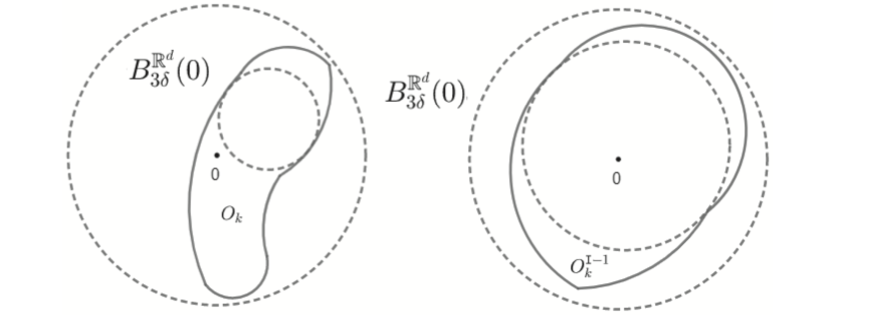
\includegraphics[width=0.62\textwidth]{figures/fig-chart-domain.png}

    \footnotesize Source: Dunson and Wu (2026), Figure 5.
  \end{center}
  \begin{itemize}
    \item every chart image remains inside \(B_{3\delta}^d(0)\)
    \item decreasing fitted noise makes the guaranteed inner ball larger
    \item samples drawn from an estimated inner ball are less likely to leave the chart
  \end{itemize}
\end{frame}

\begin{frame}{Backup: geometric RMSE}
  For a finite set \(Y=\{y_i\}_{i=1}^n\) and target \(S\subset\R^D\),
  \[
    G(Y,S)=
    \left\{\frac1n\sum_{i=1}^n\dist(y_i,S)^2\right\}^{1/2}.
  \]
  If \(Y_{\mathrm{true}}\) densely samples \(\iota(\M)\), Theorem 4 bounds
  the discrepancy between \(G(Y,Y_{\mathrm{true}})\) and
  \(G\{Y,\iota(\M)\}\).
  \begin{alertblock}{Evaluation caveat}
    \(G(Y,\iota(\M))\) measures how far estimates lie from the manifold;
    it does not alone measure whether the entire manifold is covered.
  \end{alertblock}
\end{frame}

\begin{frame}{Backup: algorithmic complexity and open questions}
  \vspace{4pt}
  \begin{center}
    \begin{tabular}{lll}
      \toprule
      Component & Main cost driver & Possible improvement\\
      \midrule
      neighborhoods & pairwise search in \(\R^D\) & approximate nearest neighbors\\
      local covariance & \(D\times D\) eigensystems & randomized/truncated SVD\\
      local GPs & repeated kernel solves & inducing points or shared factors\\
      interpolation & sequential chart coupling & parallel overlap graph\\
      \bottomrule
    \end{tabular}
  \end{center}
  \vspace{0.25cm}
  Open theory: GP contraction on estimated charts, anisotropic noise,
  boundaries, and globally calibrated uncertainty.
\end{frame}

\end{document}
